\chapter{Supplemental Information}
\label{supplementals}

% Software list/table
% DeepLabCut \href{https://github.com/DeepLabCut/DeepLabCut}
% MWorks \href{https://mworks.github.io}
% ScanImage 2016 \href{http://scanimage.vidriotechnologies.com}

\section{Supplementary Tables}
% \begin{table}[ht]
% \begin{tabularx}{\textwidth}{|l|X|}
% Use Case Navn:          & Opret Server \\
% Scenarie:               & At oprette en server med bestemte regler som tillader folk at spille sammen. More Text more text More Text \\
% \end{tabularx}
% \end{table}

\begin{table}[ht]
  \caption{Software and Available Repositories}
  \centering
  \footnotesize
  \begin{tabular}{ p{1.8cm}p{7.7cm}p{3.9cm}  }
    \toprule
    %\thead{Resource} & \thead{Source} & \thead{Publications} \\
    Resource & Source & Publications \\
    \midrule
    OpenRatBox  & https://github.com/coxlab/behavior\_rig & n.a. \\ 
                & https://github.com/coxlab/protocols & n.a. \\ 
                & https://github.com/julianarhee/trainingtracker & n.a. \\ 
    \midrule
    Custom  & https://github.com/julianarhee/morph-pov\newline 
             https://github.com/coxlab/povray & n.a.\newline \citet{Zoccolan2009} \\
    \addlinespace[0.05cm]
    POVRay  & http://www.povray.org & n.a. \\
    \addlinespace[0.05cm]
    MWorks  & https://mworks.github.io & n.a. \\
    \midrule
    Retinotopic Mapping & https://github.com/julianarhee/retinotopy-mapper\newline 
              https://github.com/zhuangjun1981/retinotopic\_mapping & n.a.\newline \citet{Zhuang2017} \\
    \midrule
    ScanImage   & http://scanimage.vidriotechnologies.com & \citet{Pologruto2003} \\ 
    \addlinespace[0.05cm]
    Custom & https://github.com/julianarhee/acquisition-tools\newline
                   https://github.com/HarveyLab/Acquisition2P\_class\newline
                   https://github.com/HarveyLab/helperFunctions & n.a.\newline n.a.\newline n.a.\\
    \midrule           
    CaImAn & https://github.com/flatironinstitute/CaImAn & \citet{Giovannucci2019}\newline \citet{Pnevmatikakis2019} \\
    \addlinespace[0.05cm]
    Suite2p & https://github.com/mouseland/suite2p & \citet{Pachitariu2017suite2p} \\
    \addlinespace[0.05cm]
    DeepLabCut   & https://github.com/DeepLabCut/DeepLabCut & \citet{Mathis2018}\newline \citet{Nath2019} \\
    \addlinespace[0.05cm]
    Scikit Learn   & https://scikit-learn.org & \citet{Pedregosa2011} \\
    \bottomrule
  \end{tabular}
  \label{tab:software}
\end{table}

\clearpage

%http://n2t.net/addgene:104488; RRID:Addgene_104488

% Data numbers 
\begin{table}[h]
  \caption{Data Summary}
  \centering
  \begin{tabular}{lllll}
    \toprule
    Stimulus & Area & Rats & FOVs & Responsive or Fit Cells   \\
    \midrule
    Moving bar & V1  & 7 & 9 & n.a.        \\
               & LM  & 7 & 9 & n.a.         \\
               & LI  & 6 & 9 & n.a.          \\
    \midrule
    Receptive Fields & V1  & 11 & 11 & 548  \\
                     & LM  & 8 & 8 & 241   \\
                     & LI  & 10 & 10 & 279    \\
    \midrule
    Gratings & V1  & 7 & 7 & 2211     \\
             & LM  & 8 & 8 & 2084     \\
             & LI  & 7 & 7 & 966     \\
    \midrule
    Objects  & V1  & 9 & 8 & 1028   \\
             & LM  & 10 & 7 & 684   \\
             & LI  & 8 & 7 & 402    \\
    \bottomrule
  \end{tabular}
  \label{tab:data_counts}
\end{table}

\clearpage

\section{Supplementary Figures}

% \section{Related to Chapter 1}
\begin{figure}[hbt!]
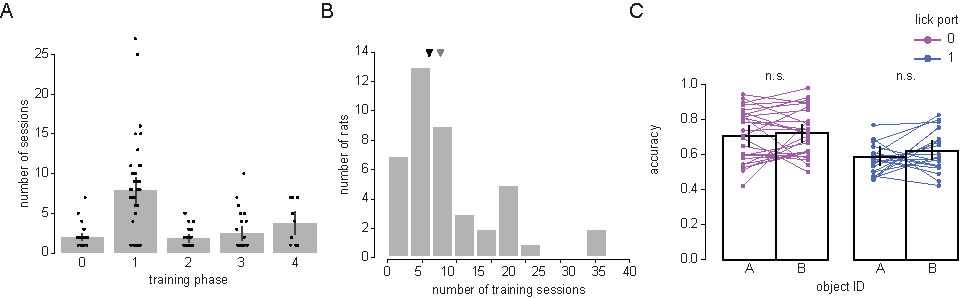
\includegraphics[width=\textwidth]{figures/supplemental/fig_s1_aggregate_training/fig_s1_aggregate_training.pdf}
    \centering
    \caption[Training timecourse for the object recognition task]{Aggregate training metrics for the visual object recognition task. 
    \textbf{A.} Number of sessions per training phase (N=48/56 rats learned the task). 0: Always Reward, 1: Default View, 2: Size Only, 3: Rotation Only, 4: Size+Rotation Cross (see Methods). Each dot represents one rat. Bars show mean and SD.
    \textbf{B.} Histogram of the total number of training sessions to reach criterion (across all phases, N=48 rats). Black and gray triangles denote the median and mean, respectively. 
    \textbf{C.} Accuracy on the discrimination task, split by object identity (object 1 or object 2) and port mapping (whether to lick right for object 1 and lick left for object 2, or vice versa). Each pair of lines represents one rat. Colors indicate arbitrary port assignment for the standard 2-object class paradigm. 
    \label{supfig:aggregate_training}}
\end{figure}

% FIGURE S.2 MORPH
\begin{figure}[hbt!]
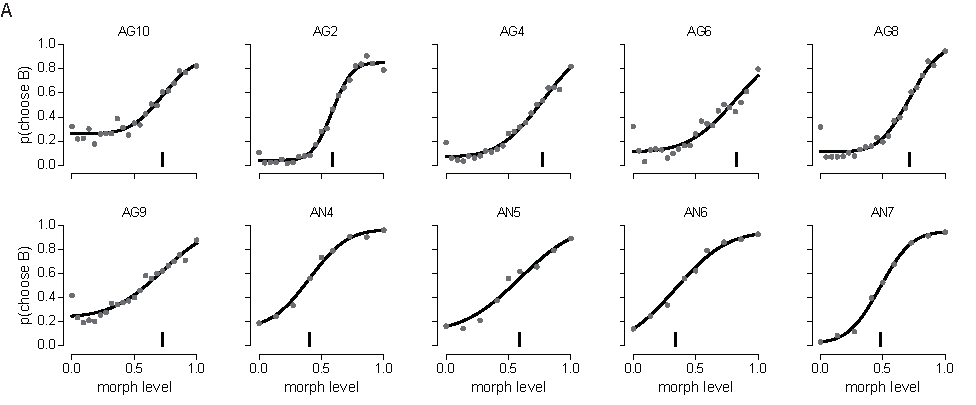
\includegraphics[width=\textwidth]{figures/supplemental/fig_s2_morphs_per_animal/fig_s2_morphs_per_animal.pdf}
    %\vspace{.1in}
    \centering
    \caption[Example psychometric curves]{Psychometric curves for rats tested on the morphs. 
    \textbf{A.} Example psychometric curves for n=10 out 13 rats that passed criterion performance (70\% accuracy on the basic discrimination of the anchors). Each dot represents the fraction of times the animal indicated that object ``B'' was presented. Morph level 0 is 0\%B and morph level 1 corresponds to 100\%B. Solid curves are the fits, vertical lines indicate the morph level of 50\% performance. 
    \label{supfig:morphs}}
\end{figure}

% FIGURE S.3 INVAR
\begin{figure}[hbt!]
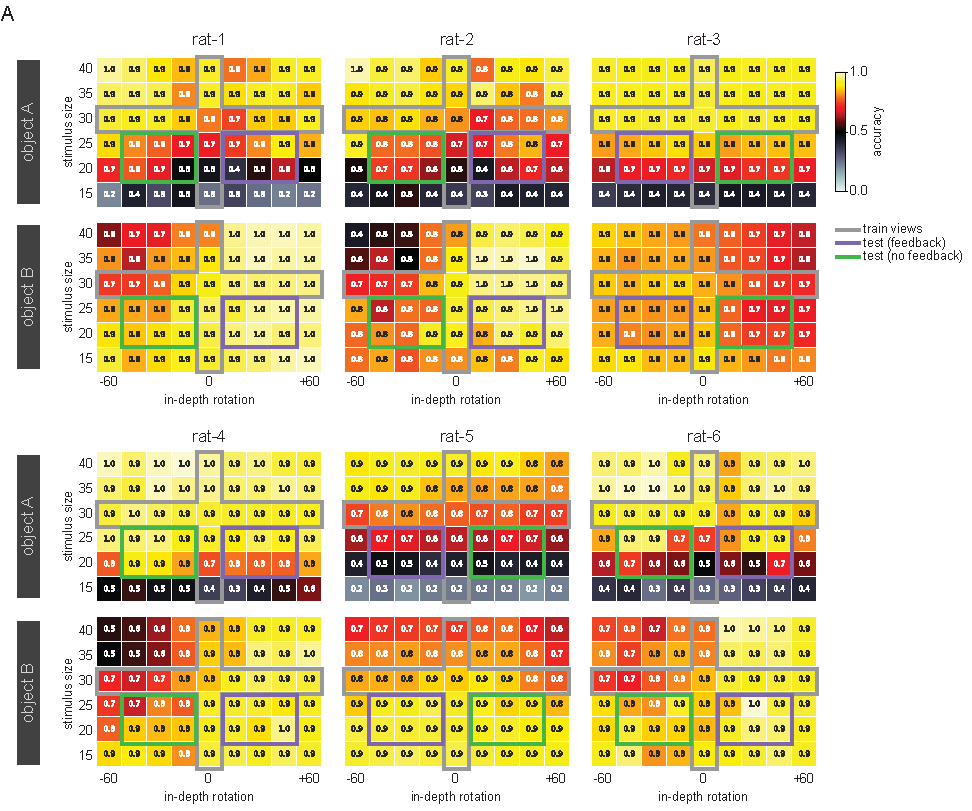
\includegraphics[width=\textwidth]{figures/supplemental/fig_s3_heatmaps_per_rat/fig_s3_heatmaps_per_rat.pdf}
    %\vspace{.1in}
    \centering
    \caption[Invariance performance for individual rats]{Example performance on the object recognition task.
    \textbf{A.} Performance data for individual rats, split by object ID (top=object A, bottom=object B) and identity-preserving transformation. Colormap indicates accuracy. Gray, initial training views (Training Phases 1-3: views in which only a single transformation axis changes, either size or rotation, see Methods). Purple, views for which no feedback was provided. Green, size-matched views for which feedback was provided. Rat-3 is the example shown in Figure\ref{fig:behavior_generalization}F.
    \label{supfig:heatmaps}}
\end{figure}

% \section{Related to Chapter 3}
% FIGURE S.4 STIMULI
\begin{figure}[t!]
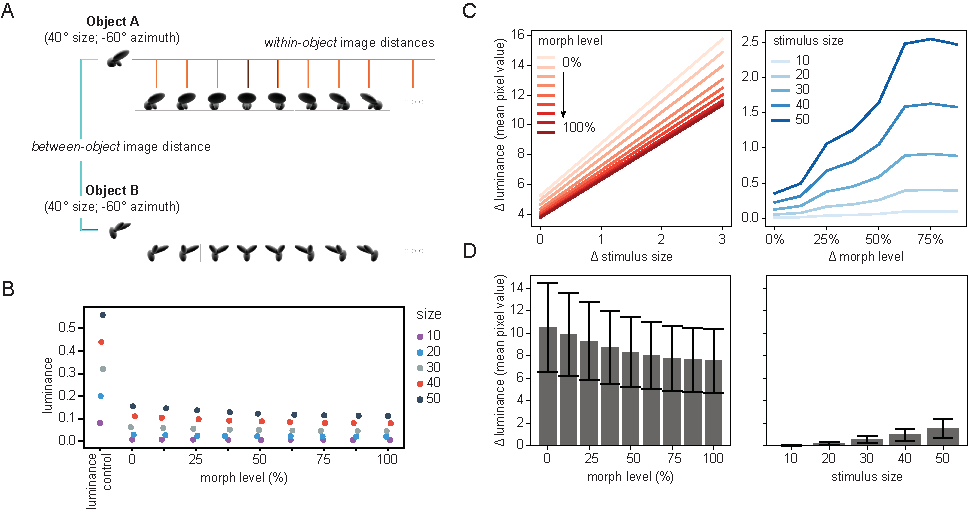
\includegraphics[width=\textwidth]{figures/supplemental/fig_s4_stimulus_metrics/fig_s4_stimulus_metrics.pdf}
    %\vspace{.1in}
    \centering
    \caption[Stimulus metrics]{Metrics for relative shape differences.
    \textbf{A.} The two objects were required to have larger within-object distances than between-object distances at a given view (adapted from \citet{Zoccolan2009}). Distance was calculated as the Euclidean distance between the images. 
    \textbf{B.} Global mean luminance for each object image used for two-photon experiments, calculated as the average pixel value across the screen (image was transformed to screen coordinates), normalized by 255 (max luminance value). Images are a subset of the stimuli used to test behavior in trained rats. Luminance controls were 5 full-field stimuli (no shapes), each assigned a constant grayscale value that was experimentally determined to match photometer measurements of the screen at each stimulus size (placed at the position of the animal's eye, see Methods). 
    \textbf{C.} \textit{Left}: Within-morph differences across different sizes. This was calculated as the pixel-wise difference between the morph $m_j$ at size $s_i$ and the same $m_j$ at size $s_{i+1}$ for each morph level, $m=9$ total morphs (level 1 represents the two smallest sizes, while level 4 represents the two largest sizes). Shades of red correspond to morph levels ordered from 0\%B to 100\%B. \textit{Right}: Between-morph differences at each size, calculated as the pixel-wise difference between morph $m_i$ and morph $m_{i+1}$ at size $s_j$ for each size ($j=5$ sizes). Differences are greater at larger sizes.
    \textbf{D.}. Average within-morph differences (across size) for each morph tested (left), and average between-morph differences (across morph levels) at each size tested (right).    
    \label{supfig:stimulus_metrics}}
\end{figure}

% Visual field targeting
\begin{figure}[hbt!]
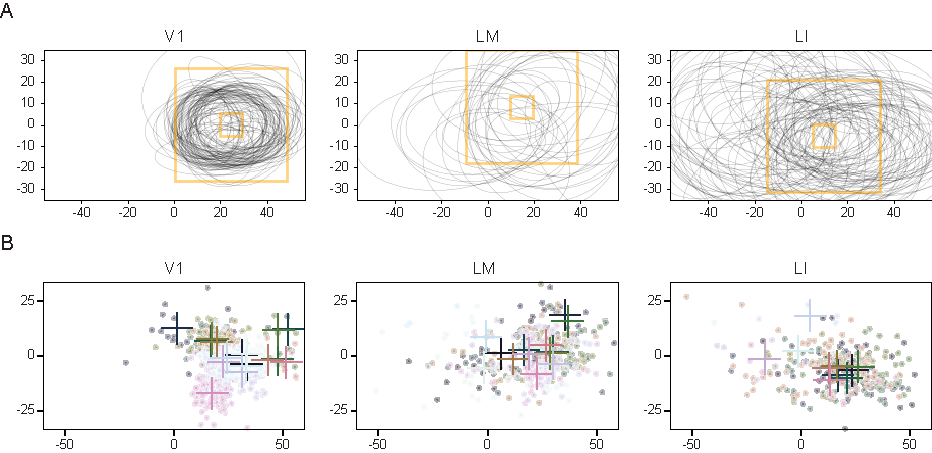
\includegraphics[width=\textwidth]{figures/supplemental/fig_s5_vf_targeting/fig_s5_vf_targeting.pdf}
    %\vspace{.1in}
    \centering
    \caption[Visual field targeting]{Targeted visual stimulation with receptive field mapping.
    \textbf{A.} Receptive fields drawn on screen coordinates for all cells in an example V1 (left), LM (middle), and LI (right) FOV. Yellow boxes correspond to bounding boxes indicating the bounds of the smallest and largest stimulus sizes targeted to the center-of-mass of the receptive fields based on localizer runs (see Methods).
    \textbf{B.} Receptive field centers (dots) and corresponding center-of-mass estimates (crosses) plotted in screen coordinates for FOVs recorded in V1 (left), LM (middle), and LI (right). Colors correpsond to different FOVs. The FOVs shown here are a subset of the object data (Chapter 4) for which cells were both visually responsive for object stimuli and had well-fit receptive fields in the same session.
    \label{supfig:vf_targeting}}
\end{figure}


% \subsection{Comparison of stimulus size for receptive field measurements}
\begin{figure}[hbt!]
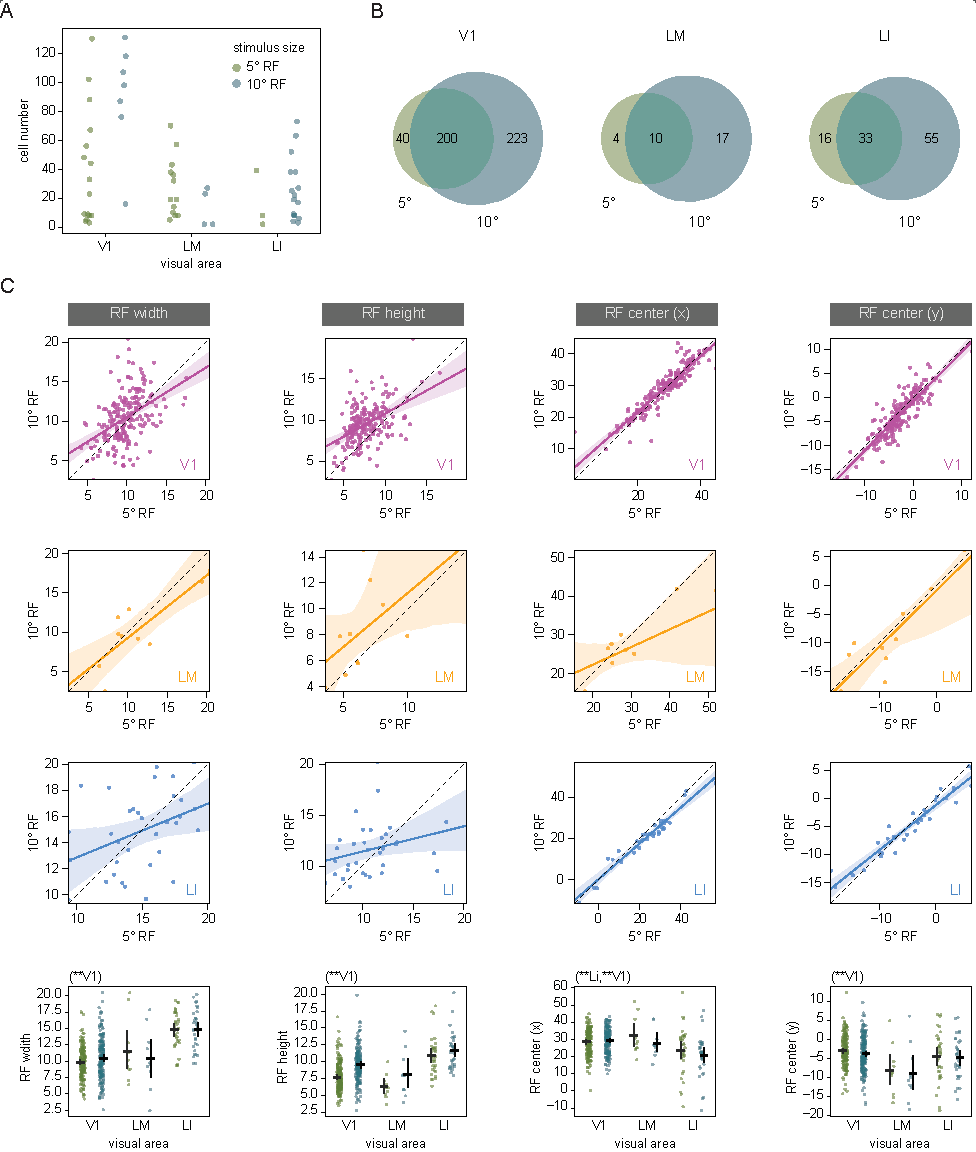
\includegraphics[width=0.9\textwidth]{figures/supplemental/fig_s6_rf5_v_rf10/fig_s6_rf5_rf10.pdf}
    %\vspace{.1in}
    \centering
    \caption[RF mapping stimulus sizes]{Comparison of receptive fields (RFs) measured with two stimulus sizes.
    \textbf{A.} Number of cells with well-fit RFs (see Methods) for \ang{5} (light green, left points) and \ang{10} (dark green, right points) stimulus sizes. Each dot is a FOV.
    \textbf{B.} RF counts for FOVs in which both sizes were tested for V1, LM, and LI. Overlap, cells fit with both sizes. Light green, \ang{5}. Dark green, \ang{10}.
    \textbf{C.} Scatter plots of RF parameters using the \ang{5} (x-axis) and \ang{10} (y-axis) for cells fit with both. Columns represent estimated parameters of the 2-D Gaussian ($\sigma_1$, $\sigma_2$, $x_0$, $y_0$). Row 1 (magenta): V, Row 2 (orange): LM, Row 3 (blue): Li. Row 4, scatterplot data plotted side-by-side for the parameter in the column (\ang{5}: light green, left, \ang{10}: dark green, right) for each area. Axis titles above Row 4 plots indicate visual areas for which there was a significant difference between sizes (Wilcoxon rank test, *:p<0.05, **:p<0.01).
    \label{supfig:rf5_rf10}}
\end{figure}

% \subsection{Comparison of stimulus size for receptive field measurements}
\begin{figure}[hbt!]
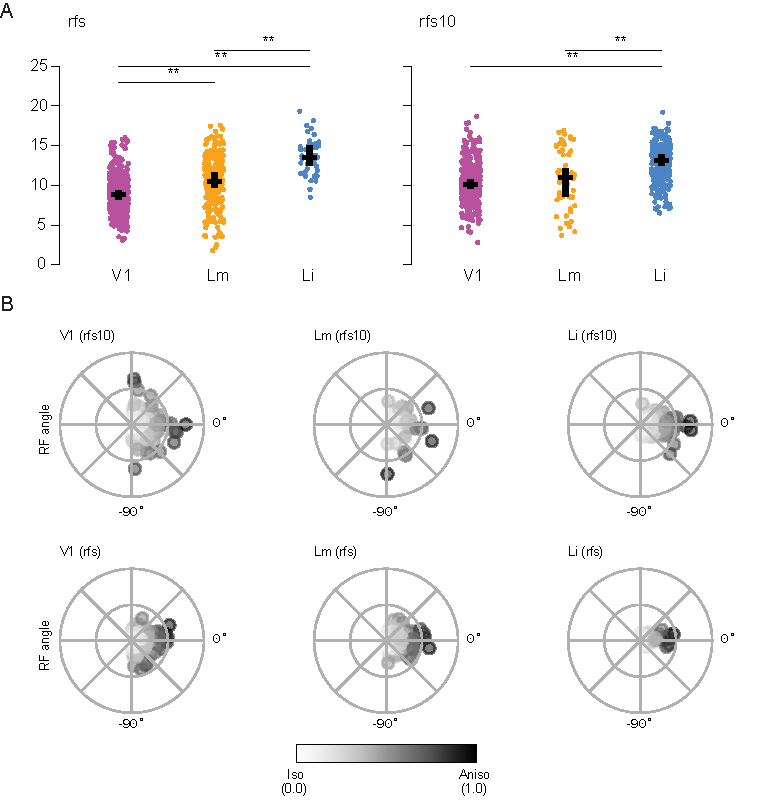
\includegraphics[width=0.8\textwidth]{figures/supplemental/fig_s7_rf5_rf10_aggregate/fig_s7_rf5_rf10_aggregate.pdf}
    %\vspace{.1in}
    \centering
    \caption[Comparison of RF metrics]{Comparison of RF metrics measured with two stimulus sizes.
    \textbf{A.} Average size (mean of $\sigma_1$ and $\sigma_2$ of the fit 2-D Gaussian, see Methods) for cells fit using a \ang{5} resolution (left) or \ang{10} resolution (right) tile size. Each dot is a cell. Black horizontal and vertical bars, mean and SD. (Mann-Whitney U-test, *p<0.05, **p<0.01, corrected for multiple comparisons with Benjamini/Hochberg).
    \textbf{B.} Anisotropy, measured as the ratio of major to minor axes of the fit ellipse, as a function of receptive field angle, for receptive fields measured at \ang{10} (top row) or \ang{5} (bottom row) tile sizes. Each dot is a cell. Anistropy ranges from 0 to 1, where 0 represents perfectly isotropic receptive fields (a circle), and 1 represents an extremely linear receptive field. Receptive field angles of 0 represent orientations parallel to the horizontal axis, and 90 degrees represents orientation parallel to the vertical axis.
    \label{supfig:rf5_rf10_aggregate}}
\end{figure}


% \subsection{Demonstration of spherical correction}
\begin{figure}[hbt!]
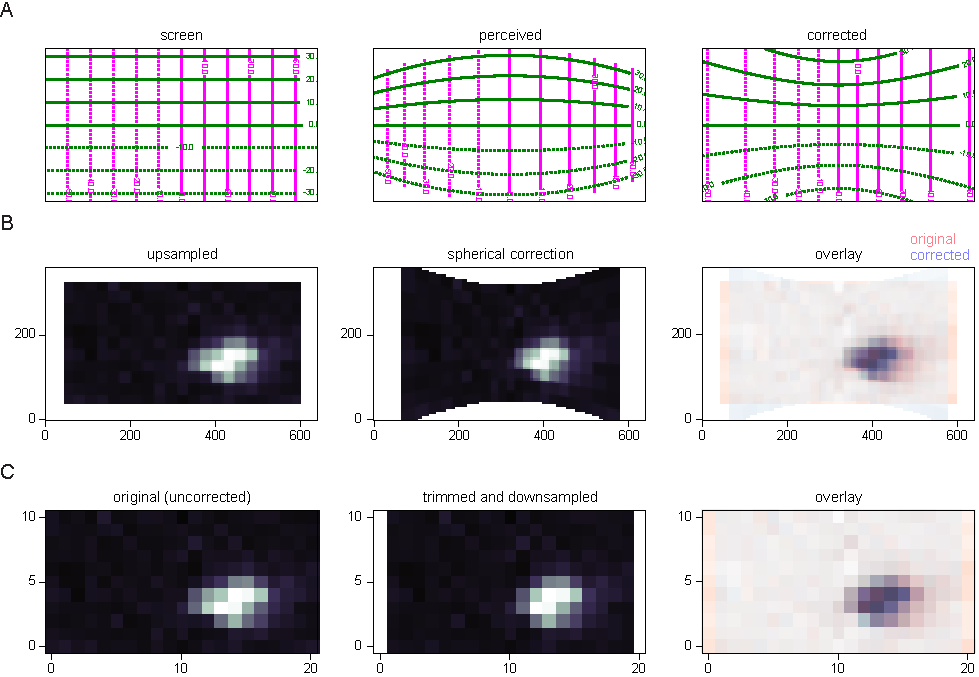
\includegraphics[width=\textwidth]{figures/supplemental/fig_s8_spherical_correction_steps/fig_s8_spherical_correction_steps.pdf}
    %\vspace{.1in}
    \centering
    \caption[Spherical correction]{Steps for applying spherical correction to RF maps.
    \textbf{A.} \textit{Left}: Screen coordinates of the monitor in degrees of visual angle. \textit{Middle}: Estimate of what the animal perceives without spherical correction\cite{Labrigger2012}. \textit{Left}: Transform to warp RF responses measured without spherically-corrected stimuli. Green, isoelevation lines. Magenta, isoazimuth. Inset numbers indicate coordinate space in degrees of visual angle.
    \textit{B.} Steps for applying a spherical correction to measured RF responses. First, the measured RF array, corresponding to the cell's average response to each stimulated position or tile, is transformed to pixel coordinates (left, downsampled screen resolution is the upsampled RF array). Then, the transformation for ``corrected'' RF maps (shown in \textbf{A}, left) is applied to the RF array (middle). The overlay (right) shows the warped RF array (blue) overlaid on the upsampled RF array (red) in pixel coordinates. Units are in pixels.
    \textbf{C.} Steps to convert spherically-corrected RF arrays back to coordinates of the tiled RF map. \textit{Left}: The original RF array showing the cell's response to each of the tiled position. \textit{Middle}:  The upsampled and warped RF array (shown in the middle panel directly above in \textbf{B}, middle) is then trimmed and downsampled back to the tiled stimulus coordinates (as opposed to the upsampled pixel coordinates). Right, overlay of the ``corrected'' RF array (blue) ontop of the original RF array (red). Units are in monitor locations of the stimulated tile positions (degrees of visual angle), where 0 is the temporal edge (azimuth) or the lower edge (elevation).
    \label{supfig:spherical_correction_steps}}
\end{figure}

% \subsection{Spherical correction, examples}
\begin{figure}[hbt!]
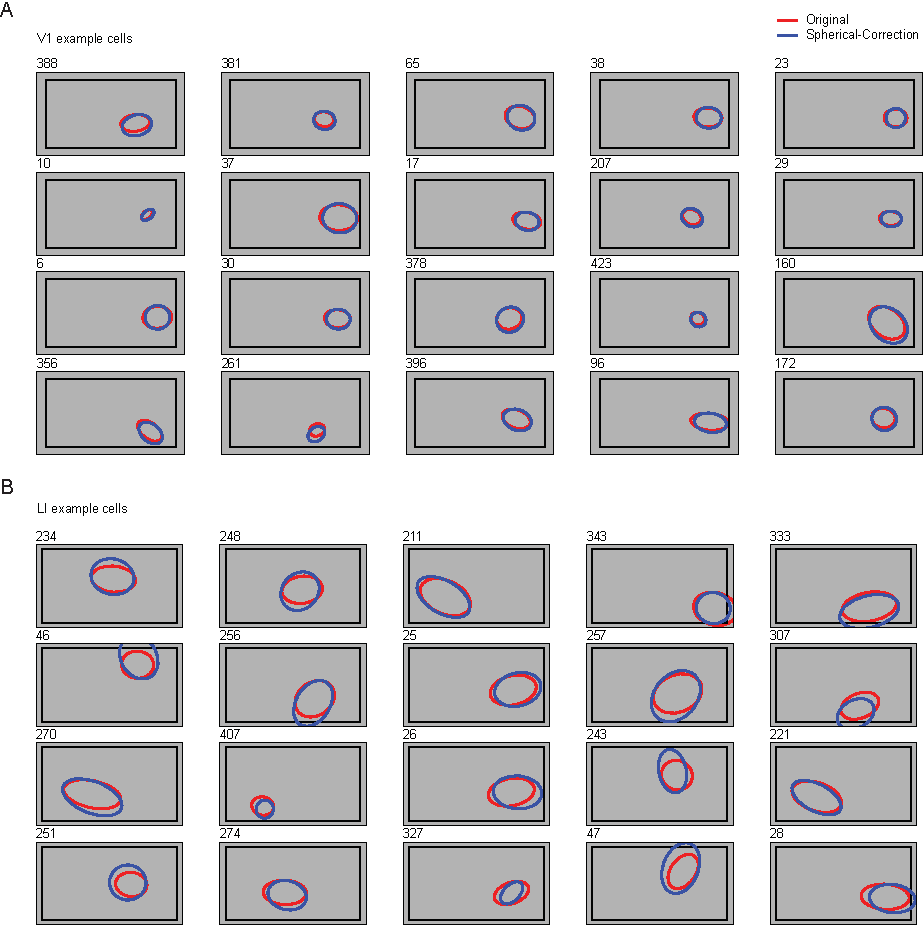
\includegraphics[width=\textwidth]{figures/supplemental/fig_s9_spherical_correction_examples/fig_s9_spherical_correction_examples.pdf}
    %\vspace{.1in}
    \centering
    \caption[Example RFs after spherical correction]{Example receptive field fits before and after spherical correction.
    \textbf{A.} Top 30 cells (ranked by goodness-of-fit measure, coefficient-of-determination $R2$) for an example V1 FOV. Red, original RF fit. Blue, RF fit after warping. 
    \textbf{B.} Same as \textbf{A}, but for an example LI FOV, where cells are generally larger and cover peripheral parts of the screen.
    \label{supfig:spherical_correction_examples}}
\end{figure}


% \subsection{Spherical correction, aggregate}
\begin{figure}[hbt!]
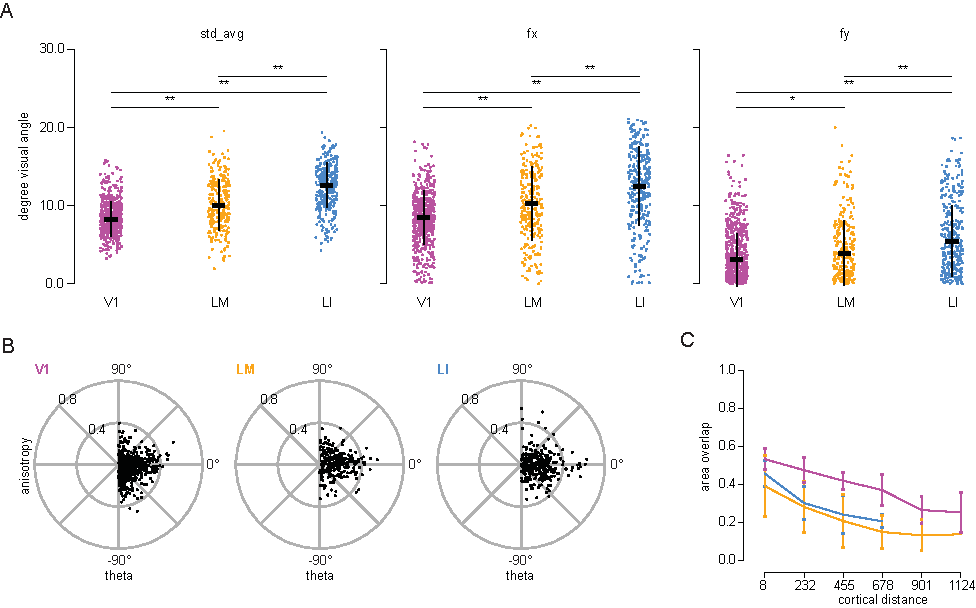
\includegraphics[width=\textwidth]{figures/supplemental/fig_s10_spherical_correction_aggregate/fig_s10_spherical_correction_aggregate.pdf}
    %\vspace{.1in}
    \centering
    \caption[RF properties with spherical correction]{RF properties after applying spherical corrections. 
    \textbf{A.} Average size (left), measured as half-width at half-max (HWHM) of a double Guassian fit. Also shown is the projection of the major axis of each ellipse onto the horizontal (middle) or vertical (right) axes of visual space for each cell. Each dot represents one cell. Horizontal and vertical bars, mean and SD across cells. 
    \textbf{B.} Anisotropy, measured as the ratio of major to minor axes of the fit ellipse, as a function of receptive field angle. Each dot is a cell. Anistropy ranges from 0 to 1, where 0 represents perfectly isotropic receptive fields (a circle), and 1 represents an extremely linear receptive field. Receptive field angles of 0 represent orientations parallel to the horizontal axis, and 90 degrees represents orientation parallel to the vertical axis.
    \textbf{C.} Receptive field overlap as a function of cortical distance. For each pair of cells, overlap is measured as the intersection of their receptive fields divided by their union. Error bars, SD. 
    \label{supfig:spherical_correction_aggregate}}
\end{figure}


% \section{Related to Chapter 4}
\begin{figure}[t!]
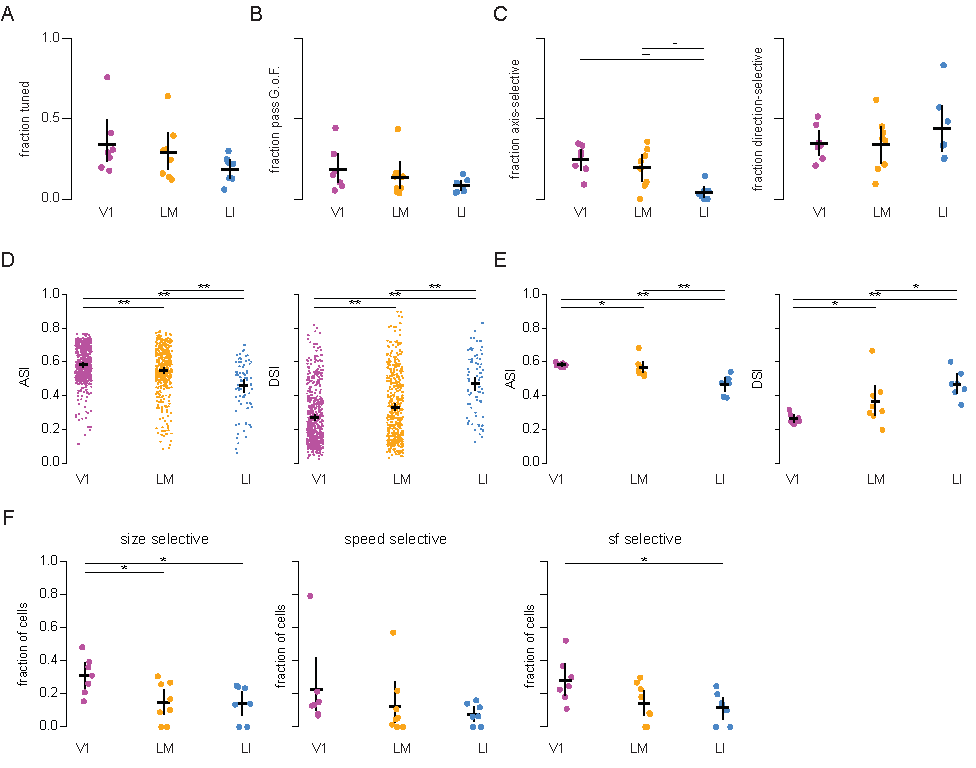
\includegraphics[width=\textwidth]{figures/supplemental/fig_s11_gratings_aggregate/fig_s11_gratings_aggregate.pdf}
    %\vspace{.1in}
    \centering
    \caption[Aggregated gratings metrics]{Summary of tuning for drifting gratings.
    \textbf{A.} Fraction of visually responsive cells tuned to gratings stimuli (significantly tuned to at least 2 stimulus conditions). Each dot represents one FOV. Black vertical and horizontal bars, mean and SD. *:p<0.05, **:p<0.01, Mann-Whitney U-test corrected for multiple comparisons (see Methods).
    \textbf{B.} Fraction of visually responsive cells that passed all goodness-of-fit (G.o.F.) criteria for direction tuning curve fits (see Methods). Each dot represents one FOV, conventions as in \textbf{A}.
    \textbf{C.} Fraction of axis-selective cells (left) and direction-selective cells (right). Conventions as in \textbf{A} and \textbf{B}.
    \textbf{D.} Distributions of ASI (left) and DSI (right) for well-fit cells. Each dot represent one cell. Black lines, mean and SD.
    \textbf{E.} Average ASI (left) and DSI (right) for each FOV. Each dot represents one imaging site.
    \textbf{E.} Fraction of cells that showed a preference for size (left), speed (middle), and spatial frequency (right). 
    \label{supfig:gratings_aggregate}}
\end{figure}

% \subsection{Comparison of receptive field and gratings tuning}
\begin{figure}[hbt!]
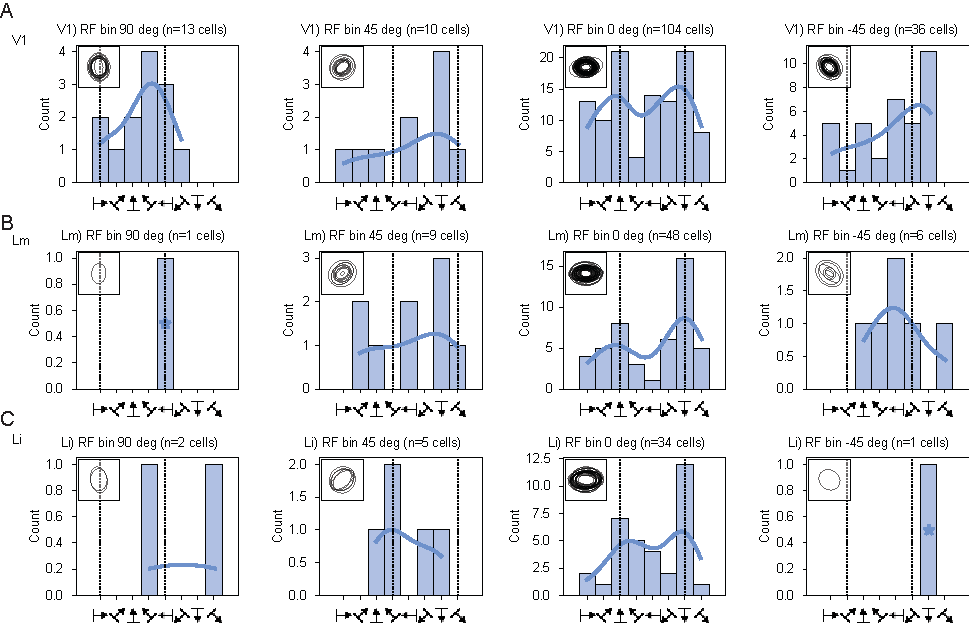
\includegraphics[width=\textwidth]{figures/supplemental/fig_s12_theta_vs_rf/fig_s12_theta_vs_rf.pdf}
    %\vspace{.1in}
    \centering
    \caption[Direction selectivity and RF orientation]{Direction selectivity by receptive field orientation.
    \textbf{A.} Distributions of preferred theta (direction of motion) for cells with well-fit direction tuning curves and well-fit RFs (see Methods), split by binned RF orientation, for V1 cells. Inset at the upper left of each subplot shows the actual RF fits for the cells whose preferred theta distributions are shown in the corresponding histogram. Solid blue curves, estimated KDEs (kernel density estimates). Dotted vertical lines, 
    \textbf{B.} Same as \textbf{A}, but for LM cells. Plots with a single star (and no KDE curve) contain only 1 cell. 
    \textbf{C.} Same as \textbf{A} and \textbf{B} for LI cells. Conventions as above.
    \label{supfig:theta_vs_rf}}
\end{figure}


% \section{Related to Chapter 4}
\begin{figure}[hbt!]
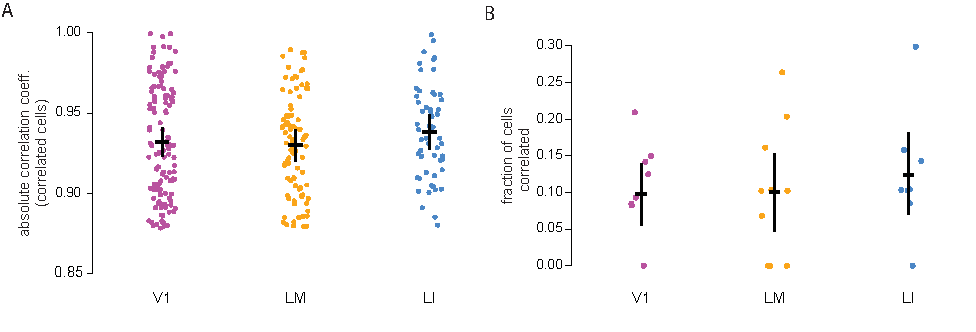
\includegraphics[width=\textwidth]{figures/supplemental/fig_s13_luminance_corr/fig_s13_luminance_corr.pdf}
    %\vspace{.1in}
    \centering
    \caption[Luminance and size tuning]{Relationship between luminance selectivity and size selectivity.
    \textbf{A.} Distributions of absolute values of correlation coefficients for cells with significant relationships between size tuning and luminance tuning (Pearson's, p<0.05) for visually responsive cells in V1, LM, and LI. Each dot represents one cell. Vertical and horizontal bars, mean and SD. 
    \textbf{B.} Fraction of cells with significant correlations for each visual area recorded in V1, LM, and LI. Each dot represents one imaging site.  
    \label{supfig:luminance_corr}}
\end{figure}



% \subsection{Tuning similarity as a function of distance}

% \subsection{Classifier accuracy as a function of receptive overlap}

% \subsection{Classifier generalization, matched for receptive field size}
